\chapter{Changements entre deux mondes}
\graphicspath{{img/chap3}}
Après avoir implémenté le monde et les règles, il faut maintenant mettre en place une stratégie d'applications de ces changements sur le monde. 
\section{File d'attente des changements}
Une méthode possible pour stocker les changements à effectuer entre deux monde est d'utiliser une file, qui sera alors défilé au besoin. Cette méthode permet de ne stocker que les changements réels à appliquer tout en conservant leur ordre d'application grâce à la structure en file.

\subsection{Représentation d'un changement par un nœud}
Avant même de travailler sur la file de changements, il faut dans un premier temps concevoir et implémenter un élément (un changement) de cette file.

Nous avons fait le choix de modéliser un changement à effectuer par un nœud de liste simplement chaînée, comportant les attributs suivants :
\begin{itemize}
    \item les coordonnées de la case à modifier;
    \item le numéro de la règle à appliquer;
    \item l'indice de l'état à appliquer à cette case;
    \item un pointeur vers un autre nœud : le nœud suivant dans la file.
\end{itemize}

En C, l'implémentation d'un tel objet se fait à l'aide de la structure suivante :
\begin{lstlisting}
struct change {
    unsigned int i, j, idx_rule, idx_next_state;
    struct change* next;
};
\end{lstlisting}
\label{lst:StructureChangement}
Cette structure est incorporée tel quel dans l'en-tête \texttt{queue.h} afin de rendre ses attributs accessibles aux autres parties du programme. Cela permet de récupérer et appliquer aisément la règle et l'état du changement.

\subsection{Structure de la file en liste chaînée}
Maintenant que l'on a modélisé les changements sous forme de nœuds, il nous suffit de les chaîner pour obtenir une liste chaînée de nœuds, que l'on pourra manipuler selon le fonctionnement d'une file.

Cette file est implémentée sous forme d'une structure avec les attributs suivants :
\begin{itemize}
    \item un tableau de changements, qui constitue l'espace de stockage des nœuds de la file;
    \item le nombre d'éléments de cette liste;
    \item le pointeur vers le premier nœud de la file des changements en attente;
    \item le pointeur vers le dernier nœud des changements en attente;
    \item le pointeur vers le premier nœud de la liste chaînée des changements déjà effectués.
\end{itemize}

Ceci donne en C l'implémentation suivante :
\begin{lstlisting}
struct queue {
    unsigned int len_list_changes;
    struct change list_changes[MAX_QUEUE_SIZE];
    struct change* first_to_do;
    struct change* first_done;
    struct change* last_to_do;
};
\end{lstlisting}
\label{lst:StructureQueue}
\clearpage
Cette file était dans un premier temps déclarée entièrement dans le \texttt{queue.h}, comme l'est la structure des changements. Cependant, afin de préserver les attributs de la file, nous avons décidé de déclarer uniquement une structure abstraite \lstinline{struct queue} dans l'en-tête \texttt{queue.h}, à l'image des règles. On ne travaille qu'avec une seule file \lstinline{struct queue queue} déclarée comme variable globale dans le code source de la file \texttt{queue.c}.

En plus de la file souhaitée, cette structure comporte une liste chaînée des changements déjà effectués. Celle-ci fait ainsi office de \og corbeille \fg{} de changements, sur lequel on peut éventuellement opérer et permet de \og  supprimer \fg{} un défilement sans devoir libérer un espace du tableau des changements de la file par allocation dynamique.

\subsection{Manipulation et optimisation de la file}
Une fois la structure de la file établie, il ne reste plus qu'à définir les méthodes permettant de manipuler la file.
Pour cela, on définit trois méthodes principales :
\begin{itemize}
    \item \lstinline{void queue_init()} pour initialiser une file déjà crée;
    \item \lstinline{int queue_is_not_empty()} qui indique si la file comporte un élément ou pas;
    \item \lstinline{void queue_append(unsigned int i, unsigned int j, unsigned int idx_rule, unsigned int idx_next_state)} pour ajouter un changement en queue d'une file existante;
    \item \lstinline{struct change* queue_pop()} pour récupérer le changement en tête de file et le supprimer de celle-ci.
\end{itemize}

Il est aussi utilisé deux fonctions supplémentaires :
\begin{itemize}
    \item \lstinline{create_change()}, utilisée par \lstinline{queue_append()} pour (dans une première version) ajouter simplement un changement dans le tableau et en définir les attributs du changement souhaité.
    \item \lstinline{queue_is_not_empty()} qui indique si une file est vide ou non.
\end{itemize}

L'initialisation d'une file se fait simplement en mettant à zéro le nombre de ses éléments et en mettant tous ses pointeurs à \lstinline{NULL}, ce qui permet de réinitialiser la file à chaque nouvelle image sans devoir effacer le contenu du tableau \lstinline{list_changes}. 

L'ajout d'un changement à la file se faisait dans un premier temps uniquement en éditant l'élément \lstinline{list_change[len_list_changes]} (comme décrit dans la \autoref{fig:QueueAppend}). Cependant, cette stratégie d'apparence simple pose rapidement des problème au niveau du tableau \lstinline{list_changes}, qui peut rapidement déborder et provoquer des erreurs de segmentations. Pour palier à cet inconvénient autrement qu'en agrandissant arbitrairement \lstinline{MAX_QUEUE_SIZE} = \lstinline{WIDTH*HEIGHT}, on réécrit les nouveaux changements en suivant la liste chaînée \og corbeille \fg{} \lstinline{first-done} dès que celle-ci possède un élément (voir \autoref{fig:QueueRemoveAfterAppend}). Ceci résout les problèmes d'espace mémoire sans augmenter la taille du tableau des changements tant qu'on opère bien un seul changement par cellule du monde, ce qui est bien le cas dans le programme principal.

\begin{figure}[ht]
\centering
\begin{subfigure}{0.45\textwidth}
    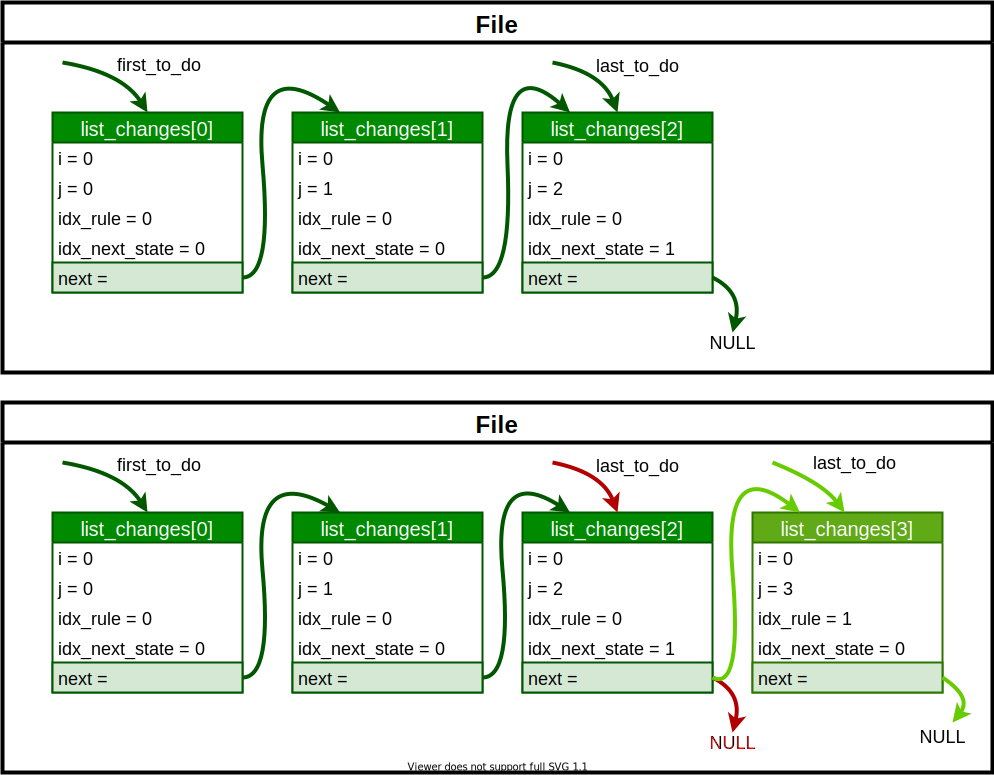
\includegraphics[width=\textwidth]{queue_append.png}
    \subcaption{Ajout d'un élément à la file}
    \label{fig:QueueAppend}
\end{subfigure}
\hfill
\begin{subfigure}{0.45\textwidth}
    \includegraphics[width=\textwidth]{queue_pop.png}
    \subcaption{Suppression d'un élément de la file}
    \label{fig:QueueRemove}
\end{subfigure}
    \caption{Fonctionnement interne de la file}
    \label{fig:Queue}
\end{figure}

\clearpage
\begin{figure}[h!]
\ContinuedFloat
    \centering
    \begin{subfigure}{0.45\textwidth}
        \includegraphics[width=\textwidth]{queue_popAfterAppend.png}
        \subcaption{Ajout d'un élément après une suppression (après optimisation)}
        \label{fig:QueueRemoveAfterAppend}
    \end{subfigure}
    \caption{Fonctionnement interne de la file (suite)}
\end{figure}

\subsection{Correction et complexités de la file}
Pour vérifier le bon comportement de la file, nous avons créé l'exécutable \texttt{test\_queue} (intégré aux tests exécutés par \texttt{makefile test}. Celui-ci permet de tester le bon fonctionnement des méthodes de la file, c'est-à-dire l'ajout, la suppression d'un changement et l'existence d'un élément dans la file ou non.. À chaque fois, on vérifie le bon nombre d'éléments et on vérifie leur bon emplacement dans l'espace mémoire, par un test et un affichage sur la sortie standard par les fonctions \lstinline{void queue_view_to_do()} et \lstinline{void change_view(struct change* change)}.

D'après ce qu'on a vu précédemment, la complexité temporelle des différentes fonctions de manipulations de la file sont constantes, puisqu'elles ne sont constituées que d'un nombre constant de manipulations de pointeurs. De même, la complexité en espace de la file ne sera caractérisée que par l'espace pris par le stockage des changements par \lstinline{list_changes}, qui est égale à la taille du monde.

En définitive, l'utilisation de cette file est de complexité temporelle constante et cette dernière possède une complexité spatiale linéaire en la taille du monde.

\section{Gestion des conflits}
On a vu précédemment que l'on parcourt chaque cellule d'un monde à chaque image pour estimer s'il y a un changement à effectuer ou pas. Cependant, dès que l'on inclut un déplacement de cases dans les règles, il peut arriver que deux cases veulent aller au même endroit à l'image suivante, ce qui pose problème. Ces situations constituent des conflits, que l'on doit gérer.

\subsection{Marquage d'un conflit}
Gérer un conflit commence d'abord par le détecter. Pour cela, on utilise un tableau de la taille du monde qui stocke le nombre de cellules qui souhaitent se déplacer vers une autre. On conserve également le nombre de conflits restant à gérer. Un conflit est ainsi implémentée en C par la structure suivante :
\begin{lstlisting}
struct conflict {
    unsigned int nb_conflicts;          //Nombre de cellules devant aller à celle-ci
    unsigned int conflict_to_process;   //Nombre de conflits à gérer/appliquer
};
\end{lstlisting}

Marquer l'ensemble des conflits d'un monde revient alors à créer un tableau de \lstinline{struct conflict}

Ensuite, il suffit d'incrémenter ces valeurs dès qu'une case doit se déplacer sur une cellule vide. Si la case d'arrivée n'est pas vide, la particule ne peut pas se déplacer, il n'y a donc pas de conflit. On obtient alors la détection des conflits suivante, au sein même de \texttt{project.c}~:
\begin{lstlisting}
if ((w.t[index_tmp] == EMPTY && (dx_tmp || dy_tmp)) || (!(dx_tmp || dy_tmp)) {
    t_conflicts[index_tmp].nb_conflicts += 1;
    t_conflicts[index_tmp].conflict_to_process += 1;
    queue_append(k, l, j, idx_change);
} else {
    fprintf(stderr, "Conflit perdant en %d %d car déplacement dans une case non vide.\n", k + dx_tmp, j = dy_tmp);
}
\end{lstlisting}
On remarque alors que l'ajout d'un changement à la file dépendant de l'état de la case d'arrivée. Si elle est vide, un changement est ajouté à la file. Si elle ne l'est pas, la cellule de départ reste inchangée. Ceci constitue donc déjà un début de résolution de conflit.

\subsection{Résolution des conflits} \label{sec:Conflits}
Un fois les conflits sauvegardés, on les résout au moment de vider la file et d'appliquer les changements.

Pour cela, on regarde pour chaque changement combien de conflits concerne la case où doit s'appliquer le changement :
\begin{itemize}
    \item Si la case n'a pas de conflit, alors on n'applique pas le changement, la cellule ayant déjà été modifiée ;
    \item Si la case ne comporte qu'une seule cellule voulant s'installer là, il n'y a pas de conflit et alors le changement est appliqué ;
    \item Si la case comporte plus d'une cellule voulant se déplacer là, alors on effectue un tirage au sort (suivant une loi uniforme ; $\frac{1}{\texttt{nb\_conflict}}$) pour appliquer ou non le changement :
    \begin{itemize}
    \item Si le tirage est gagné, alors la cellule est marquée comme n'ayant plus de conflit et on on applique le changement ;
    \item Sinon, la case est marquée comme ayant une cellule en moins à gérer et on n'applique pas le changement.
    \end{itemize}
\end{itemize}
Dans notre programme, c'est la fonction \lstinline{solve_conflict()} qui conditionne l'application d'un changement par \lstinline{world_apply_rule()} :
\begin{lstlisting}
int solve_conflict(struct conflict t_conflicts[], unsigned int i, unsigned int j)
{
    struct conflict c = t_conflicts[i * WIDTH + j];
    int random = rand();
    if (c.nb_conflicts == 0) { //conflit déjà résolu
        return 0;
        fprintf(stderr, "Conflit perdant en %d %d car nb_conflicts =0\n", i, j);
    } else if (c.conflict_to_process == 1) { // conflit à résoudre avec ce changement
        return 1;
    } else if ((random % c.nb_conflicts) == 0) { // changement gagnant
        t_conflicts[i * WIDTH + j].nb_conflicts = 0;
        return 1;
    } else { // changement perdant
        t_conflicts[i * WIDTH + j].conflict_to_process -= 1;
        return 0;
    }
}
\end{lstlisting}
Enfin, il suffit d'appliquer le conflit si \lstinline{solve_conflict} retourne 1. Pour cela, on change la cellule de destination selon le changement à appliquer et on rend la cellule de départ vide s'il y a eu un déplacement. La fonction \lstinline{world_apply_rule} devient alors :

\clearpage
\begin{lstlisting}
void world_apply_rule(struct world* w, struct rule* r, int i, int j,
    unsigned int idx_change, struct conflict t_conflicts[])
{
    unsigned int dx = rule_change_dx(r, idx_change);
    unsigned int dy = rule_change_dy(r, idx_change);
    int s = solve_conflict(t_conflicts, modulo(i + dx, HEIGHT), modulo(j + dy, WIDTH));
    if (s) { //si la résolution de conflit dit qu'on doit appliquer le changement
        if (dx || dy) { // il y a déplacement
            w->t[modulo(i + dx, HEIGHT) * WIDTH + modulo(j + dy, WIDTH)] = rule_change_to(r, idx_change);
            w->t[i * WIDTH + j] = DEAD; // la cellule de départ est vide
        } else { // changement de couleur uniquement
            w->t[i * WIDTH + j] = rule_change_to(r, idx_change);
        }
    }
}
\end{lstlisting}

\subsection{Correction et efficacité de la gestion des conflits}
La résolution des conflits se faisant de manière aléatoire, il est difficile d'automatiser les tests pour vérifier si les conflits sont biens gérés comme tel. Nous avons donc choisi de faire un test simplement \og visuel \fg{}, en recréant un monde simple mettant en situation un conflit entre deux cellules voulant aller au même endroit, de manière cyclique au fur et à mesure des images. En générant un grand nombre d'images et donc de conflits, on doit pouvoir apercevoir le caractère aléatoire de la résolution de conflit. Les résultats de ces tests sont illustrés 
\autoref{fig:TestConflict}
\begin{figure}[ht]
    \centering
    \begin{subfigure}{0.2\textwidth}
        \includegraphics[width=\textwidth]{TestConflict1.png}
        \subcaption{Création d'un conflit entre deux cellules allant au centre}
        \label{fig:TestConflict1}
    \end{subfigure}
    \hfill
    \begin{subfigure}{0.2\textwidth}
        \includegraphics[width=\textwidth]{TestConflict2.png}
        \subcaption{Victoire de la cellule jaune, attente de la cellule verte}
        \label{fig:TestConflict2}
    \end{subfigure}
    \hfill
    \begin{subfigure}{0.2\textwidth}
        \includegraphics[width=\textwidth]{TestConflict3.png}
        \subcaption{Attente de la cellule verte car case d'arrivée non-vide}
        \label{fig:TestConflict3}
    \end{subfigure}
    \hfill
    \begin{subfigure}{0.2\textwidth}
        \includegraphics[width=\textwidth]{TestConflict4.png}
        \subcaption{Victoire de la case verte dans la situation vu en \autoref{fig:TestConflict1}}
        \label{fig:TestConflict4}
    \end{subfigure}
    \caption{Tests de la résolution des conflits}
    \label{fig:TestConflict}
\end{figure}

Pour ce qui est de l'efficacité de la résolution des conflits, notre implémentation semble cohérente au reste de notre programme. En effet, nous ne parcourons jamais le tableau des conflits en entier (ce qui permet de garder les avantages temporaires de la file). De plus, les conflits sont stockés lors de l'ajout à la file et les conflits sont résolus lors des défilements des changement. On en déduit que la complexité spatiale de la résolution n'est uniquement impactée par le tableau de marquage des conflits, qui possède la même taille que le monde. De plus, la résolution ne nécessite aucune boucle, puisqu'elle ne fait que décider d'une application d'un changement ou non. Au final, on en déduis que la complexité de la gestion des conflits est constante en temps et linéaire en espace suivant la taille du monde.